\documentclass[11pt,a4paper]{article}
\usepackage{fullpage}
\usepackage{tabu}
\usepackage[utf8]{inputenc}
\usepackage{tikz}
\usepackage{pgf}
\usetikzlibrary{arrows,automata}
\usetikzlibrary{positioning}
\title{Beastly Heis v1.5}
\author{Kolbjørn Austreng, Andreas Våge}

\tikzset{
    state/.style={
           rectangle,
           rounded corners,
           draw=black, very thick,
           minimum height=2em,
           inner sep=2pt,
           text centered,
           },
}

\begin{document}
\maketitle
\section*{Diagrams}
\begin{figure}[h]
\centering
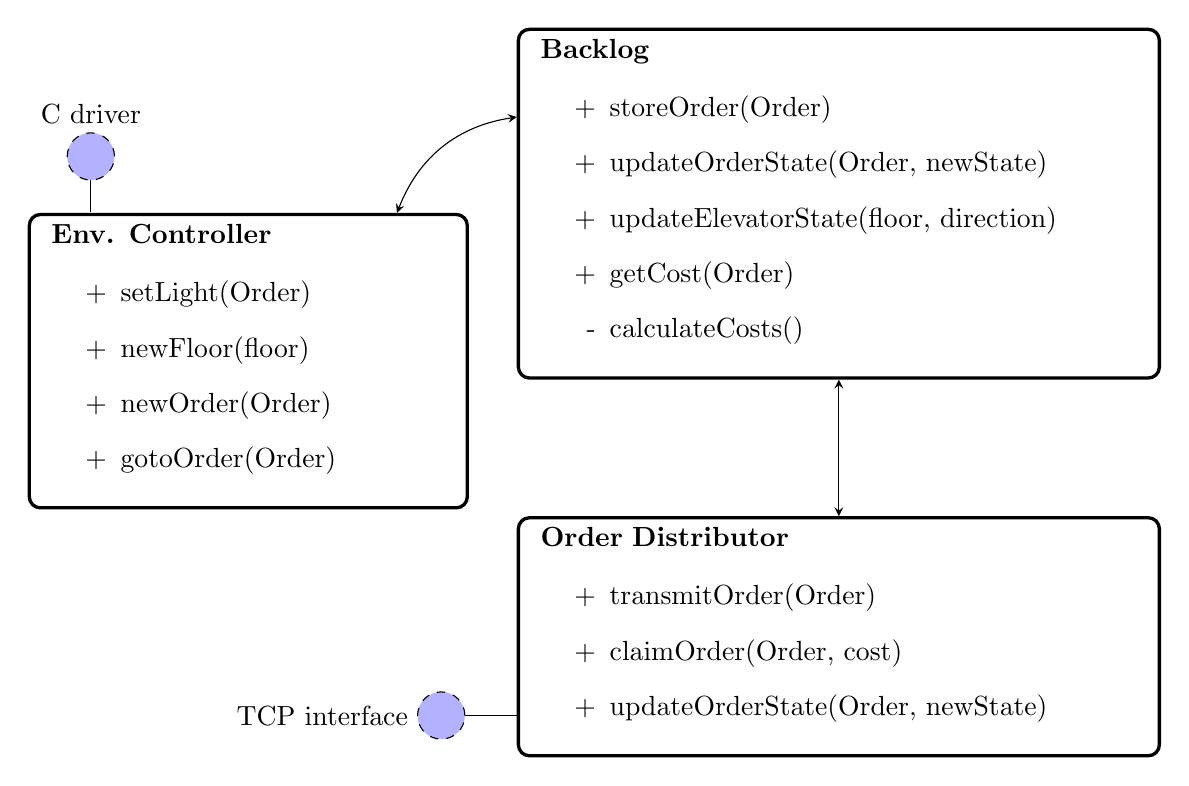
\begin{tikzpicture}[->,>=stealth]

 % Position of Env Controller 
 % Use previously defined 'state' as layout (see above)
 % use tabular for content to get columns/rows
 % parbox to limit width of the listing
 \node[state] (Env Controller)
 {\begin{tabular}{l}
  \textbf{Env. Controller}\\
  \parbox{5cm}{\begin{itemize}
   \item[+] setLight(Order)
	\item[+] newFloor(floor)
	\item[+] newOrder(Order)
	\item[+] gotoOrder(Order)
  \end{itemize}
  }
 \end{tabular}};

 \node[state,       % layout (defined above)
  text width=8cm,   % max text width
  yshift=2cm,       % move 2cm in y
  right of=Env Controller,   
  node distance=7.5cm,  
  anchor=center] (Backlog)  % posistion relative to the center of the 'box'
  {\begin{tabular}{l}
  \textbf{Backlog}\\
  \parbox{8cm}{\begin{itemize}
   \item[+] storeOrder(Order)
   \item[+] updateOrderState(Order, newState)
   \item[+] updateElevatorState(floor, direction)
   \item[+] getCost(Order)
   \item[-] calculateCosts()

  \end{itemize}
  }
 \end{tabular}};
 
 % STATE Communication
 \node[state,
  below of=Backlog,
  yshift=-4.5cm,
  anchor=center,
  text width=8cm] (Communication) 
 {\begin{tabular}{l}
  \textbf{Order Distributor}\\
  \parbox{8cm}{\begin{itemize}
   \item[+] transmitOrder(Order)
   \item[+] claimOrder(Order, cost)
   \item[+] updateOrderState(Order, newState)

  \end{itemize}
  }
 \end{tabular}};

 
 % draw the paths and and print some Text below/above the graph
 \path[<->] (Env Controller)  edge[bend left=30]   (Backlog)
 %(Env Controller)        edge[bend right=20]  (Communication)
 %(Communication)     edge[loop below]    node[anchor=north,below]{$SC_n\neq 0$} (Communication)
 (Communication)     edge                 (Backlog);

% Tacked on orbital data
\begin{scope}[-]
\begin{scope}[xshift=0.8cm,yshift=-0.4cm]
\path[draw] (-2.8,2.3) -- (-2.8,3);
\path[draw,dashed, fill = blue!30] (-2.8, 3) circle (0.3) node[above = 0.3cm] {C driver};
\end{scope}
\path[draw] (3.45,-4.5) -- (2.45,-4.5);
\path[draw,dashed, fill = blue!30] (2.45,-4.5) circle (0.3) node[left = 0.3cm] {TCP interface};
\end{scope}
\end{tikzpicture}
\caption{System module diagram.}
\end{figure}
\begin{figure}[h]
\centering
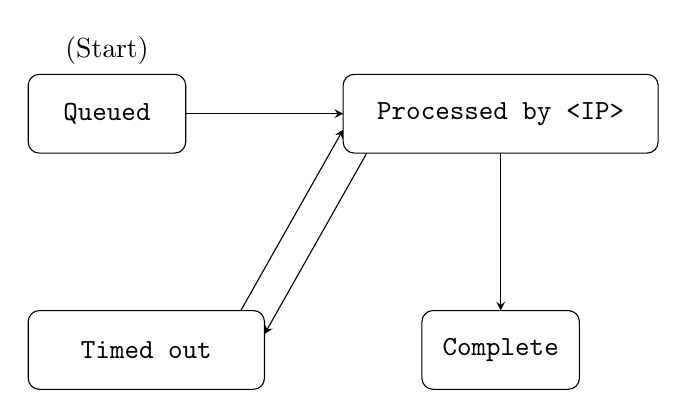
\begin{tikzpicture}[>=stealth]
\path[draw, rounded corners, fill = white] (0,4) rectangle (2,5) node[midway] {\verb!Queued!};
\path[draw, rounded corners, fill = white] (4,4) rectangle ++(4,1) node[midway] {\verb!Processed by <IP>!};
\path[draw, rounded corners, fill = white] (0,1) rectangle ++(3,1) node[midway] {\verb!Timed out!};
\path[draw, rounded corners, fill = white] (5,1) rectangle ++(2,1) node[midway] {\verb!Complete!};
\path[draw,->] (2,4.5) -- ++(2,0);
\path[draw,->] (6, 4) -- ++(0,-2);
\path[draw,->] (4.3,4) -- (3,1.7);
\path[draw,->] (2.7,2) -- (4,4.3);
\path (1,5) node[above] {(Start)};
\end{tikzpicture}
\caption{Order life stages.}
\end{figure}
\section*{Order object}
\begin{tabu}{|X|X|}
\hline
\textbf{Order} & Comment\\ \hline
+ type & Internal / External\\
+ floor & Destination floor\\
+ timestamp & Set by computer that first received order\\
+ origin IP & Set by computer that first received order\\
+ state & Queued, In progress, Timed out, Complete\\ \hline
\end{tabu}
\section*{Environment Controller}
\subsubsection*{+ setLight(Order)}
Sets the light corresponding to the floor of an Order object.
\subsubsection*{+ newFloor(int floor)}
Call from C driver to communicate to \textit{Environment Controller} that a new floor has been reached.
\subsubsection*{+ newOrder(Order)}
Call from C driver to communicate to \textit{Environment Controller} that a new order has been created.
\subsubsection*{+ gotoOrder(Order)}
Sends the elevator to the floor of a specific order.
\section*{Backlog}
\subsubsection*{+ storeOrder(Order) ok}
Saves an order from either \textit{Environment Controller} or \textit{Order Distributor} to the backlog. Returns acknowledgement.
\subsubsection*{+ updateOrderState(Order, newState) ok}
Changes the state of a specific order. Returns acknowledgement.
\subsubsection*{+ updateElevatorState(int floor, enum direction}
Communicates the position and direction of the elevator to the \textit{Backlog}.
\subsubsection*{+ getCost(Order) cost}
Returns the cost of taking a specific order for this elevator.
\subsubsection*{- calculateCosts()}
Calculates the costs of all the orders in the backlog for this elevator.
\section*{Order Distributor}
\subsubsection*{+ transmitOrder(Order) ok}
Transmits an Order object to all the other nodes in the network. Acknowledges if at least one other elevator received the order transmit, or there are no other elevators in the network.
\subsubsection*{+ claimOrder(Order, cost) ok}
Attempts to claim an order in the \textit{Backlog}. Transmits own cost of taking on this order. Acknowledges if no other elevators have a lower cost on the specified order.
\subsubsection*{+ updateOrderState(Order, newState) ok}
Broadcasts an order state update to ensure that the backlogs are identical.
\end{document}